\documentclass{standalone}
\usepackage{tikz}
\begin{document}
            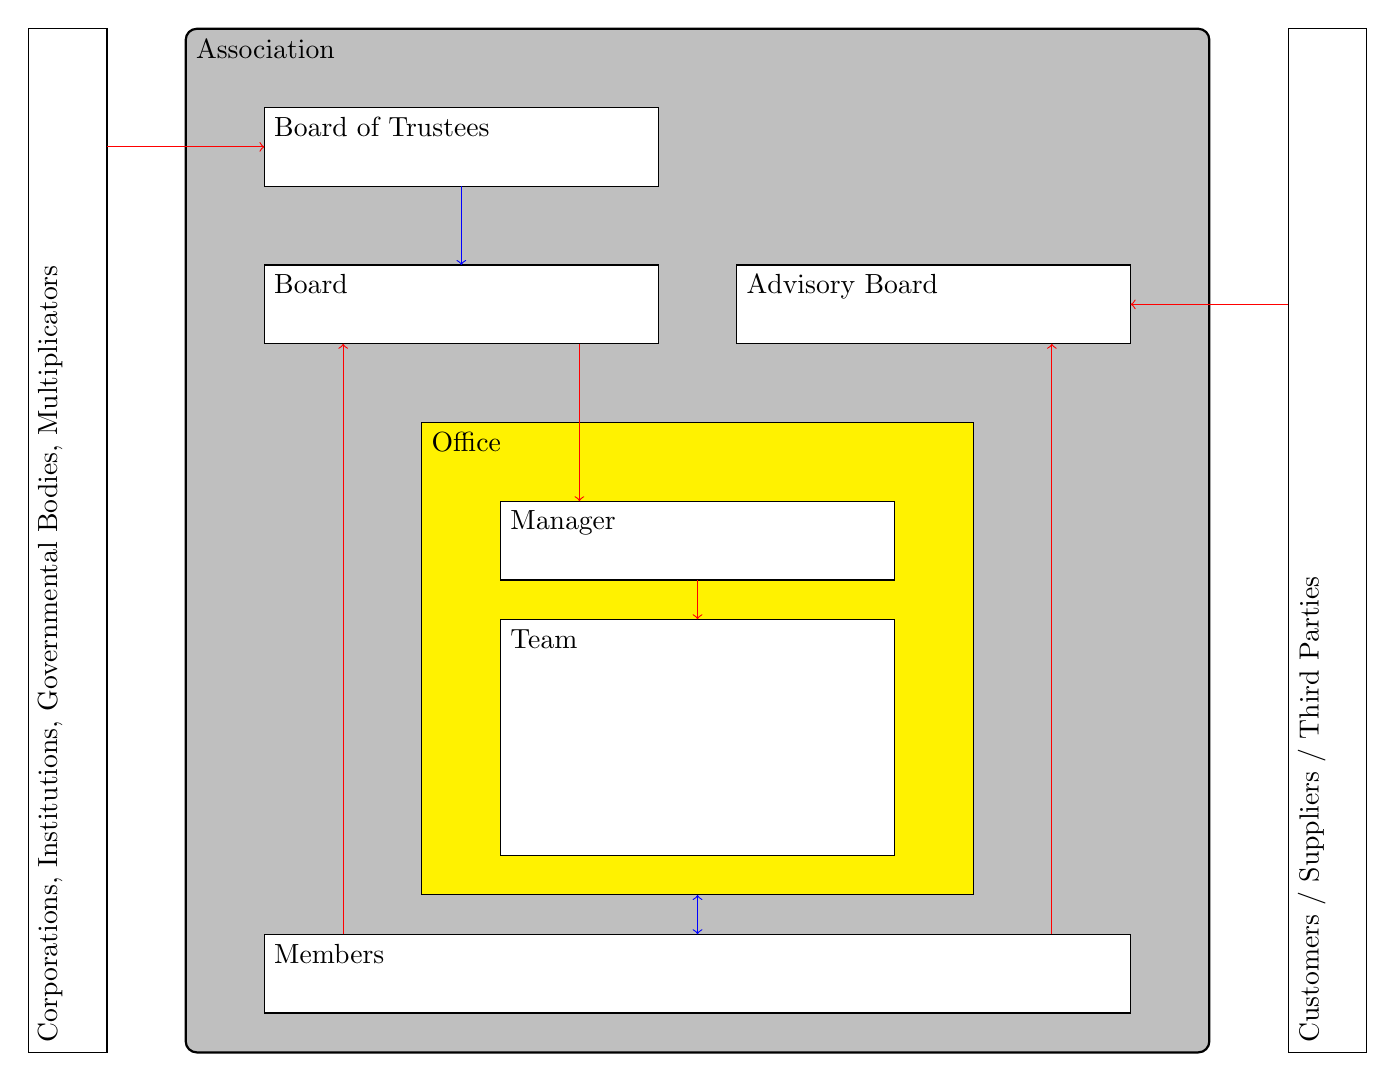
\begin{tikzpicture}
            \draw[thick,rounded corners,fill=lightgray] (3,2) node[below right] {Association} rectangle (16,-11);
            \draw[fill=white] (4,1) node[below right] {Board of Trustees} rectangle (9,0);
            \draw[fill=white] (4,-1) node[below right] {Board} rectangle (9,-2);
            \draw[fill=white] (10,-1) node[below right] {Advisory Board} rectangle (15,-2);
            \draw[fill=yellow] (6,-3) node[below right] {Office}
            rectangle (13,-9);
            \draw[fill=white] (7,-4) node[below right] {Manager} rectangle (12,-5);
            \draw[fill=white] (7,-5.5) node[below right] {Team} rectangle (12,-8.5);
            \draw[fill=white] (4,-9.5) node[below right] {Members} rectangle (15,-10.5);
            \draw (17,-11) node[below right,rotate=90] {Customers / Suppliers / Third Parties} rectangle (18,2);
            \draw (1,-11) node[below right,rotate=90] {Corporations, Institutions, Governmental Bodies, Multiplicators} rectangle (2,2);
            \draw[color=red,->] (2,0.5) -- (4,0.5); % körpersch-kurat
            \draw[color=red,->] (5,-9.5) -- (5,-2); % mitgl-vorst
            \draw[color=blue,->] (6.5,0) -- (6.5,-1); % kurat-vorst
            \draw[color=red,->] (8,-2) -- (8,-4); % vorst-netzw
            \draw[color=red,->] (9.5,-5) -- (9.5,-5.5); % netzw-mita
            \draw[color=blue,<->] (9.5,-9.5) -- (9.5,-9); %mitgl-koo
            \draw[color=red,->] (17,-1.5) -- (15,-1.5); % bild-fachbei
            \draw[color=red,->] (14,-9.5) -- (14,-2); % mitgl-fachbei
            % \draw[fill=white] (11.5,-6.5) node[below right] {Advisory Board}
            % rectangle (15,-7.5);
        \end{tikzpicture}
\end{document}